
%(BEGIN_QUESTION)
% Copyright 2007, Tony R. Kuphaldt, released under the Creative Commons Attribution License (v 1.0)
% This means you may do almost anything with this work of mine, so long as you give me proper credit

{\it Limit switches} are electrical switches designed to actuate based on the motion or position of an object, rather than the touch of a human operator.  Simple limit switches rely on direct, physical contact, using a lever, sometimes tipped with a roller for low friction:

$$\includegraphics[width=15.5cm]{i02242x01.eps}$$

\vskip 30pt

Show how you would connect the limit switch in the above illustration so that it makes the light turn {\it off} when actuated (i.e. the light will be on when no one touches the switch lever).

\underbar{file i02242}
%(END_QUESTION)





%(BEGIN_ANSWER)

$$\includegraphics[width=15.5cm]{i02242x02.eps}$$

%(END_ANSWER)





%(BEGIN_NOTES)


%INDEX% Switch, limit: mechanical actuation (direct contact)

%(END_NOTES)


